\documentclass[tikz,border=5pt]{standalone}
\usetikzlibrary{arrows.meta,positioning}
\begin{document}
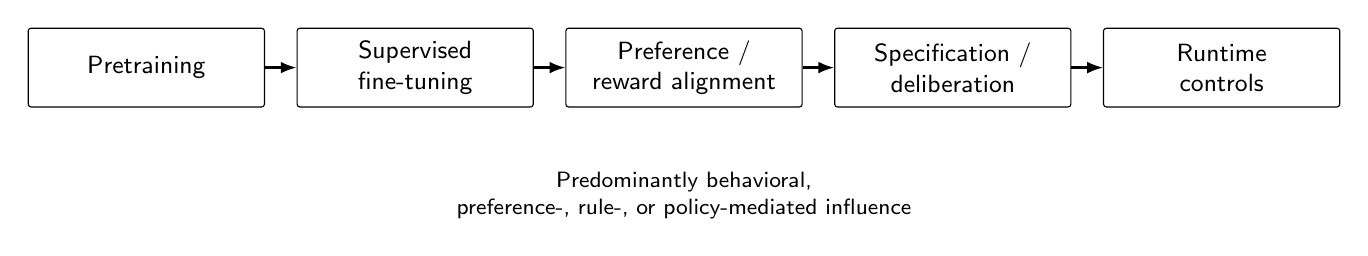
\begin{tikzpicture}[
  node distance=5mm and 4mm,
  box/.style={draw, rounded corners=1pt, minimum width=30mm, minimum height=10mm, align=center, font=\sffamily\small},
  arrow/.style={-{Latex[length=2mm]}, thick}
]
\node[box] (pre) {Pretraining};
\node[box, right=of pre] (sft) {Supervised\\fine-tuning};
\node[box, right=of sft] (pref) {Preference /\\reward alignment};
\node[box, right=of pref] (spec) {Specification /\\deliberation};
\node[box, right=of spec] (run) {Runtime\\controls};
\draw[arrow] (pre) -- (sft);
\draw[arrow] (sft) -- (pref);
\draw[arrow] (pref) -- (spec);
\draw[arrow] (spec) -- (run);
\node[below=7mm of pref, align=center, font=\sffamily\footnotesize] {Predominantly behavioral,\\preference-, rule-, or policy-mediated influence};
\end{tikzpicture}
\end{document}
